\chapter{IAPWS-97 thermodynamics}
\label{iapws97}
\index{thermodynamics!IAPWS-97}
\index{PyTOUGH!thermodynamics!IAPWS-97}

\section{Introduction}
The \texttt{IAPWS97} library in PyTOUGH contains a Python implementation of the main functions of the International Association for the Properties of Water and Steam 1997 (IAPWS-97) thermodynamic formulation \citep{iapws_2000}.  These can be used to calculate the thermodynamic properties of water, steam and supercritical water.  The IAPWS-97 supersedes the IFC-67 formulation used in TOUGH2 (see section \ref{t2thermo}), being generally faster and more accurate, as well as having a simpler representation of the thermodynamic region around the critical point.

The operating range of the IAPWS-97 formulation is shown in the pressure-temperature plot below.  It covers temperatures up to 800 $\degree$C and pressures up to 100 MPa, and is divided into four thermodynamic regions:

\begin{enumerate}
  \item liquid water
  \item dry steam
  \item supercritical fluid
  \item two-phase
\end{enumerate}

The two-phase region (4) follows the saturation line on the pressure-temperature plot (the boundary between liquid water and dry steam), up to the critical point $C$ ($T$ = 373.946 $\degree$C, $P$ = 22.064 MPa), where the distinction between liquid water and steam disappears.  Region 3 covers supercritcal fluid (above the critical point) and also near-critical fluid, just below the critical point.  The boundary between regions 1 and 3 (liquid water and supercritical) is aribitrarily set at $T$ = 350 $\degree$C.  The boundary between regions 2 and 3 (dry steam and supercritical) is described by the \texttt{b23p} and \texttt{b23t} functions, given in section \ref{region23_boundary}.

\index{thermodynamics!IAPWS-97!operating range}
\begin {figure}
  \begin{center}
    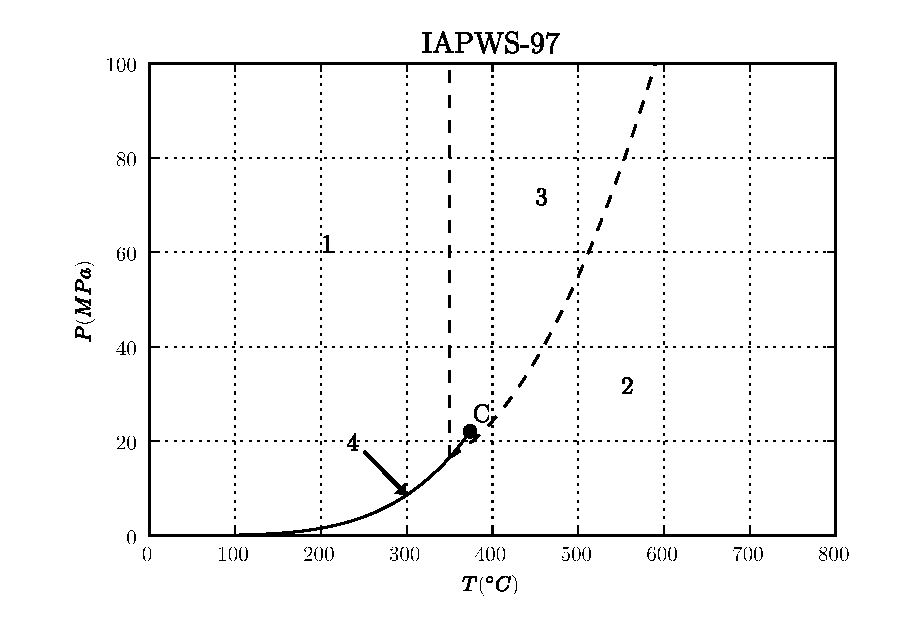
\includegraphics{ptplot.eps}
    \caption{Operating range of the IAPWS-97 thermodynamic formulation}
    \label{fg:iapws97_range}
  \end{center}
\end {figure}

The \texttt{IAPWS97} library can be imported using the command:

\begin{lstlisting} 
   from IAPWS97 import *
\end{lstlisting}

The functions available through the \texttt{IAPWS97} library are listed in Table \ref{tb:iapws97_functions} and described below.

\index{thermodynamics!IAPWS-97!functions}
\begin{table}
  \begin{center}
    \begin{tabular}{|l|l|p{65mm}|}
      \hline
      \textbf{Function} & \textbf{Type} & \textbf{Description}\\
      \hline
      \hyperref[sec:iapws97:b23p]{\texttt{b23p}} & float & pressure on boundary between steam and supercritical regions, as a function of temperature\\
      \hyperref[sec:iapws97:b23t]{\texttt{b23t}} & float & temperature on boundary between steam and supercritical regions, as a function of pressure\\
      \hyperref[sec:iapws97:cowat]{\texttt{cowat}} & tuple & density and internal energy of liquid water\\
      \hyperref[sec:iapws97:density_temperature_plot]{\texttt{density\_temperature\_plot}} & -- & draws region boundaries on a density-temperature plot\\
      \hyperref[sec:iapws97:pressure_temperature_plot]{\texttt{pressure\_temperature\_plot}} & -- & draws region boundaries on a pressure-temperature plot\\
      \hyperref[sec:iapws97:region]{\texttt{region}} & integer & thermodynamic region\\
      \hyperref[sec:iapws97:sat]{\texttt{sat}} & float & saturation pressure as a function of temperature\\
      \hyperref[sec:iapws97:super]{\texttt{super}} & tuple & pressure and internal energy of supercritical fluid\\
      \hyperref[sec:iapws97:supst]{\texttt{supst}} & tuple & density and internal energy of dry steam\\
      \hyperref[sec:iapws97:tsat]{\texttt{tsat}} & float & saturation temperature as a function of pressure\\
      \hyperref[sec:iapws97:visc]{\texttt{visc}} & float & dynamic viscosity of water, steam or supercritical fluid\\
      \hline
    \end{tabular}
    \caption{\texttt{IAPWS97} functions}
    \label{tb:iapws97_functions}
  \end{center}
\end{table}

\section{Thermodynamic functions}

The IAPWS-97 formulation provides thermodynamic functions for liquid water, dry steam and supercritical fluid.  These functions calculate secondary parameters from the primary thermodynamic variables.

\begin{snugshade}
\subsection{Liquid water: \texttt{cowat(\emph{t,p})}}
\end{snugshade}
\label{sec:iapws97:cowat}
\index{thermodynamics!IAPWS-97!liquid water properties}

The \texttt{cowat} function returns a two-element tuple (\texttt{d},\texttt{u}) of density (kg/m$^3$) and internal energy (J/kg) of liquid water as a function of temperature \texttt{t} ($\degree$C) and pressure \texttt{p} (Pa).

\textbf{Parameters:}
\begin{itemize}
\item \textbf{t}: float\\
  Temperature ($\degree$C)
\item \textbf{p}: float\\
  Pressure (Pa)
\end{itemize}

\begin{snugshade}
\subsection{Dry steam: \texttt{supst(\emph{t,p})}}
\end{snugshade}
\label{sec:iapws97:supst}
\index{thermodynamics!IAPWS-97!dry steam properties}

The \texttt{supst} function returns a two-element tuple (\texttt{d},\texttt{u}) of density (kg/m$^3$) and internal energy (J/kg) of dry steam as a function of temperature \texttt{t} ($\degree$C) and pressure \texttt{p} (Pa).

\textbf{Parameters:}
\begin{itemize}
\item \textbf{t}: float\\
  Temperature ($\degree$C)
\item \textbf{p}: float\\
  Pressure (Pa)
\end{itemize}

\begin{snugshade}
\subsection{Supercritical fluid: \texttt{super(\emph{d,t})}}
\end{snugshade}
\label{sec:iapws97:super}
\index{thermodynamics!IAPWS-97!supercritical fluid properties}

The \texttt{super} function returns a two-element tuple (\texttt{p},\texttt{u}) of pressure (Pa) and internal energy (J/kg) of supercritical fluid as a function of density \texttt{d} (kg/m$^3$) and temperature \texttt{t} ($\degree$C).

\textbf{Parameters:}
\begin{itemize}
\item \textbf{d}: float\\
  Density (kg/m$^3$)
\item \textbf{t}: float\\
  Temperature ($\degree$C)
\end{itemize}

\begin{snugshade}
\section{Viscosity: \texttt{visc(\emph{d,t})}}
\end{snugshade}
\label{sec:iapws97:visc}
\index{thermodynamics!IAPWS-97!viscosity}

The \texttt{visc} function returns the dynamic viscosity (Pa.s) of liquid water, dry steam or supercritical fluid as a function of density \texttt{d} (kg/m$^3$) and temperature \texttt{t} ($\degree$C).  This function is based on the supplementary ``IAPWS Formulation 2008 for the Viscosity of Ordinary Water Substance'', without the critical enhancement of viscosity near the critical point.

\textbf{Parameters:}
\begin{itemize}
\item \textbf{d}: float\\
  Density (kg/m$^3$)
\item \textbf{t}: float\\
  Temperature ($\degree$C)
\end{itemize}

\section{Region boundaries}

These functions describe the boundaries between the four thermodynamic regions of the IAPWS-97 formulation (see Figure \ref{fg:iapws97_range}).  There is no equation for the boundary between regions 1 and 3 as this is simply the line $T = 350 \degree$C.

\subsection{Saturation line: \texttt{sat(\emph{t})} and \texttt{tsat(\emph{p})}}

\begin{snugshade}
\subsubsection{\texttt{sat(\emph{t})}}
\end{snugshade}
\label{sec:iapws97:sat}
\index{thermodynamics!IAPWS-97!saturation line}

The \texttt{sat} function returns the saturation pressure (Pa) at a given temperature \texttt{t} ($\degree$C), for temperatures below the critical temperature.

\textbf{Parameters:}
\begin{itemize}
\item \textbf{t}: float\\
  Temperature ($\degree$C)
\end{itemize}

\begin{snugshade}
\subsubsection{\texttt{tsat(\emph{p})}}
\end{snugshade}
\label{sec:iapws97:tsat}
\index{thermodynamics!IAPWS-97!saturation line}

The \texttt{tsat} function returns the saturation temperature ($\degree$C) at a given pressure \texttt{p} (Pa), for pressures below the critical pressure.

\textbf{Parameters:}
\begin{itemize}
\item \textbf{p}: float\\
  Pressure (Pa)
\end{itemize}

\subsection{Steam/supercritical boundary}
\label{region23_boundary}

\begin{snugshade}
\subsubsection{\texttt{b23p(\emph{t})}}
\end{snugshade}
\label{sec:iapws97:b23p}
\index{thermodynamics!IAPWS-97!region boundaries}

The \texttt{b23p} function returns the pressure (Pa) on the boundary of the dry steam and supercritical regions (regions 2 and 3) at a given temperature \texttt{t} ($\degree$C).

\textbf{Parameters:}
\begin{itemize}
\item \textbf{t}: float\\
  Temperature ($\degree$C)
\end{itemize}

\begin{snugshade}
\subsubsection{\texttt{b23t(\emph{p})}}
\end{snugshade}
\label{sec:iapws97:b23t}
\index{thermodynamics!IAPWS-97!region boundaries}

The \texttt{b23t} function returns the temperature ($\degree$C) on the boundary of the dry steam and supercritical regions (regions 2 and 3) at a given pressure \texttt{p} (Pa).

\textbf{Parameters:}
\begin{itemize}
\item \textbf{p}: float\\
  Pressure (Pa)
\end{itemize}

\section{Determining thermodynamic region}

\begin{snugshade}
\subsubsection{\texttt{region(\emph{t}, \emph{p})}}
\end{snugshade}
\label{sec:iapws97:region}
\index{thermodynamics!IAPWS97!region}

Returns the thermodynamic region (integer, or \texttt{None}) corresponding to the given temperature ($\degree$C) and pressure (Pa), as defined by the IAPWS-97 specification. The regions are:

\begin{enumerate}
  \item liquid water
  \item dry steam
  \item supercritical
\end{enumerate}

If the input temperature and/or pressure are outside the operating range of the IAPWS-97 formulation, the routine will return \texttt{None}.

\textbf{Parameters:}
\begin{itemize}
\item \textbf{t}: float\\
  Temperature ($\degree$C)
\item \textbf{Pressure}: float\\
  Pressure (Pa)
\end{itemize}

\section{Plotting functions}

The \texttt{IAPWS97} library contains two functions used for including the IAPWS-97 thermodynamic region boundaries on plots.

\begin{snugshade}
\subsection{\texttt{pressure\_temperature\_plot(\emph{plt})}}
\end{snugshade}
\label{sec:iapws97:pressure_temperature_plot}
\index{thermodynamics!IAPWS-97!pressure-temperature plots}

Draws the IAPWS-97 thermodynamic region boundaries on a pressure-temperature diagram.

\textbf{Parameters:}
\begin{itemize}
\item \textbf{plt}: \texttt{matplotlib.pyplot} instance\\
  An instance of the \texttt{matplotlib.pyplot} library, imported in the calling script using e.g. \texttt{import matplotlib.pyplot as plt}.
\end{itemize}

\begin{snugshade}
\subsection{\texttt{density\_temperature\_plot(\emph{plt})}}
\end{snugshade}
\label{sec:iapws97:density_temperature_plot}
\index{thermodynamics!IAPWS-97!density-temperature plots}

Draws the IAPWS-97 thermodynamic region boundaries on a density-temperature diagram.  (This function requires the Scientific Python (\texttt{scipy}) library to be installed.)

\textbf{Parameters:}
\begin{itemize}
\item \textbf{plt}: \texttt{matplotlib.pyplot} instance\\
  An instance of the \texttt{matplotlib.pyplot} library, imported in the calling script using e.g. \texttt{import matplotlib.pyplot as plt}.
\end{itemize}
